%==============================================================================
% Voorbeeld gebruik documentklasse hogent-article
%==============================================================================
%
% Compileren in TeXstudio:
%
% - Zorg dat Biber de bibliografie compileert (en niet Biblatex)
%   Options > Configure > Build > Default Bibliography Tool: "txs:///biber"
% - F5 om te compileren en het resultaat te bekijken.
% - Als de bibliografie niet zichtbaar is, probeer dan F5 - F8 - F5
%   Met F8 compileer je de bibliografie apart.
%
% Als je JabRef gebruikt voor het bijhouden van de bibliografie, zorg dan
% dat je in ``biblatex''-modus opslaat: File > Switch to BibLaTeX mode.

\documentclass{hogent-article}

\usepackage{lipsum} % Voor vultekst

%------------------------------------------------------------------------------
% Metadata over het artikel
%------------------------------------------------------------------------------

%---------- Titel & auteur ----------------------------------------------------

% TODO: geef werktitel van je eigen voorstel op
\PaperTitle{De impact van het bespelen van een instrument op de wiskundige geletterdheid}
% TODO: geef op welk soort artikel dit is
% Dit is typisch de opdracht en het vak waarvoor dit artikel geschreven is, bv.
% ``Verslag onderzoeksproject Onderzoekstechnieken 2018-2019''
\PaperType{Verslag onderzoeksproject Onderzoekstechnieken 2020-2021}

% TODO: vul je eigen naam in als auteur, geef ook je emailadres mee!
\Authors{Arshad Aysha\textsuperscript{1}, Bouazzaoui Houssam\textsuperscript{2}, Moons Sebastiaan\textsuperscript{3}, Stevens Bram\textsuperscript{4}, Vanhoucke Dré\textsuperscript{5}} % Authors

% TODO: vul de naam van je co-promotor in.
% Als het hier gaat om een voorstel voor de bachelorproef, dan ben je hier
% verplicht de naam van je co-promotor in te vullen. Zoniet, dan kan je het
% leeg laten.
\CoPromotor{}

% Contactinfo: Geef hier de contactgegevens van elke auteur van het artikel (en
% indien van toepassing ook van de co-promotor).
\affiliation{
  \textsuperscript{1} \href{mailto:aysha.arshad@student.hogent.be}{aysha.arshad@student.hogent.be}}
\affiliation{
  \textsuperscript{2} \href{mailto:houssam.bouazzaoui@student.hogent.be}{houssam.bouazzaoui@student.hogent.be}}
\affiliation{
    \textsuperscript{3} \href{mailto:sebastiaan.moons@student.hogent.be}{sebastiaan.moons@student.hogent.be}}
\affiliation{
    \textsuperscript{4} \href{mailto:bram.stevens@student.hogent.be}{bram.stevens@student.hogent.be}}
\affiliation{
    \textsuperscript{5} \href{mailto:dre.vanhoucke@student.hogent.be}{dre.vanhoucke@student.hogent.be}}

%---------- Abstract ----------------------------------------------------------

\Abstract{
Wiskundige geletterdheid helpt mensen om de juiste beslissingen te nemen en om wiskunde te gebruiken en interpreteren op manieren die van belang zijn voor een denkend en betrokken individu. Al jaren wordt de correlatie tussen wiskunde en muziek gesuggereerd.
Hiervoor is de volgende onderzoeksvraag opgesteld: Heeft het bespelen van een instrument invloed op de wiskundige geletterdheid?
Het doel van dit onderzoek is om na te gaan of het bespelen van een instrument daadwerkelijk de wiskundige geletterdheid positief beïnvloedt. Om een antwoord te kunnen geven op de onderzoeksvraag werd een enquête afgenomen bij 217 studenten van de Hogeschool Gent. Hieruit werden enkele variabelen gekozen die de basis vormden van het onderzoek. De resultaten van het onderzoek impliceren dat er wel degelijk een verband is tussen het bespelen van een instrument en de wiskundige geletterdheid. De conclusie van dit onderzoek kan van belang zijn bij het het aanmoedigen van muzikale opvoeding in scholen of het opstellen van het curriculum . In de toekomst zal meer onderzoek moet worden verricht om het verband tussen wiskundige geletterdheid en het bespelen van een instrument nog meer bloot te leggen.
}

%---------- Onderzoeksdomein en sleutelwoorden --------------------------------
% TODO: Vul de sleutelwoorden aan.


\Keywords{Wiskundige geletterdheid; Instrument; Notenleer; Voorbereiding}
\newcommand{\keywordname}{Sleutelwoorden} % Defines the keywords heading name

%---------- Titel, inhoud -----------------------------------------------------

\begin{document}

\flushbottom % Makes all text pages the same height
\maketitle % Print the title and abstract box
\tableofcontents % Print the contents section
\thispagestyle{empty} % Removes page numbering from the first page

%------------------------------------------------------------------------------
% Hoofdtekst
%------------------------------------------------------------------------------

\section{Inleiding}

In deze studie wordt er nagegaan welke invloed het bespelen van een muziekinstrument heeft op de wiskundige geletterdheid. Wiskundige geletterdheid slaat op de bekwaamheid van een individu om wiskunde toe te passen, te formuleren en te begrijpen in verschillende omstandigheden. Dit is zeker de moeite waard om te onderzoeken omdat een muziekinstrument bespelen en wiskundig gerelateerde scores niet direct een verband tonen, al heeft muziek en wiskunde wel heel wat gemeenschappelijke manieren van werken. Zoals je bij muziek ook stapsgewijs te werk moet gaan met notenleer, partituren lezen, toepassen van de gelezen partituren en het bespelen van het instrument, doet dit zich dat bij wiskunde voor in de vorm van het leren rekenen, formules leren lezen en uitwerken, toepassen van de gekende leerstof op verscheidene situaties en vraagstukken oplossen.

Als data voor dit onderzoek wordt er een bevraging van de tweedejaarsstudenten van het jaar 2019-2020 Toegepaste Informatica te HoGent gebruikt. De variabelen waar er op toegespitst wordt zullen zowel het gespeelde instrument evenals de muzikale opleiding inhouden. Dit zal gaan over de aantal jaren dat het individu bezig is met muziek, het bespelen van een instrument en de kennis die men beschikt over het lezen en begrijpen van partituren. Er wordt gekeken welke invloed deze hebben op de scores van het vak Probleem Oplossend Denken, Math4IT en de scores op hun wiskundige vakken in het secundair. Ook wordt er gekeken of de muzikale achtergrond invloed heeft op het voorbereidend werk bij wiskunde gerelateerde testen

\section{Overzicht literatuur}

% Refereren naar de literatuur kan met:
% \autocite{BIBTEXKEY} -> (Auteur, jaartal)
% \textcite{BIBTEXKEY} -> Auteur (jaartal)

Er zijn al studies gevoerd naar de verbanden tussen de muzikale achtergrond en academische indicatoren om zo goed mogelijk academische wetenschappelijke prestaties te kunnen voorspellen \autocite{Brown2017}. Er was hier echter alleen maar een verband gevonden tussen de Grade Point Average en de uitkomst van academische wetenschappelijke prestatie. Dit gaat tegen het verwachte resultaat van deze studie in. De resultaten zijn echter niet compleet accuraat vanwege het lage steekproef aantal en lage betrouwbaarheid van de bevraging. Er was echter wel een positieve associatie tussen muzikale training en academische prestatie op school in een breder spectrum. Dit was zowel zichtbaar op de academische resultaten evenals een variëteit van gestandaardiseerde testen. Dit is in lijn met de andere onderzoeken die gebruikt worden.

In een Canadees onderzoek werd bekeken welke verschillen er bestaan tussen de prestaties van studenten die geëngageerd zijn met muziek en de prestaties van studenten die niet geëngageerd zijn met muziek \autocite{Boyd2013}. Er werd een verschil gemaakt tussen instrumentale muziek en enkel vocale muziek.
Het besluit uit dit onderzoek was dat er een positieve associatie is tussen geëngageerd zijn met muziek en wiskunde. De leerlingen die geëngageerd zijn met instrumentale muziek haalden de beste resultaten. De vocale groep haalden ook betere resultaten dan de leerlingen die niet geëngageerd zijn met muziek.
Het viel ook op dat leerlingen die al langer bezig zijn met muziek beter scoorden dan leerlingen die minder lang bezig waren.
Uit het onderzoek werd geconcludeerd dat leerlingen betere resultaten halen op wiskunde als ze ook geëngageerd zijn met muziek. Muziekbezigheid heeft dus een positieve associatie op wiskunde.

Uit het onderzoek van een Amerikaanse leerkracht uit Georgia bleek dat leerlingen betere wiskundige prestaties behaalden indien ze een muziekinstrument bespeelden \autocite{Sanders2018}.
Er werden verschillende soorten muziekinstrumenten onderscheiden van elkaar, namelijk vocaal, koperblazers, houtblazers en slagwerk.
Het onderzoek besloot dat muziek weldegelijk een positieve invloed heeft op wiskundige resultaten.
Hoe langer men met muziek bezig is, hoe beter de resultaten.
Enkele nulhypotheses werden aanvaard. Zo bleek dat de scores van studenten die houtblazers en slagwerk spelen geen significant verschil hadden met de scores andere studenten. Volgens de onderzoeker is dit omdat de leerlingen die deze instrumenten bespelen nog minder lang bezig zijn met muziek dan de leerlingen die andere instrumententen bespelen.
Onder andere hierdoor komt men op het besluit dat we pas echt een duidelijk verschil zien vanaf dat de leerlingen 3 jaar of langer bezig zijn met muziek.

An Song, Mary Margaret Capraro en Daniel A. Tillman hebben een onderzoek uitgevoerd of er een effect is op de studenten hun wiskundige prestaties door invloed van muzikale activiteiten \autocite{An2013}. De resultaten waren positief waardoor men kon concluderen dat de muzikale activiteiten een invloed hebben op de wiskundige prestaties van studenten. Aan het onderzoek zijn er wel beperkingen. Ten eerste, er was maar een interventieperiode van slechts 5 weken. Ten tweede, er werd doelbewust één klas leerlingen uit zowel de eerste als derde graad van een basisschool geselecteerd, waardoor de bevindingen mogelijk niet generaliseerbaar zijn voor andere leerlingen met verschillende achtergronden.

Franse onderzoekers hebben onderzocht hoe de hersenen structureel veranderen wanneer iemand voor lange tijd een muziekinstrument bespeelt \autocite{Groussard2014}. Ze hebben mensen van dezelfde leeftijd en academische achtergrond in geregelde intervallen een hersenscan laten ondergaan. Daaruit blijkt dat hoe langer iemand een muziekinstrument bespeelt hoe meer grijze hersenmassa groeit. Een grotere hoeveelheid grijze hersenmassa is positief voor de intelligentie. Ook blijkt dat bepaalde gebieden in de hersenen eerder beïnvloed worden dan andere. Het soort instrument blijkt een verwaarloosbare invloed te hebben. De data die in ons onderzoek gebruikt zal worden bevat mensen die al enkele jaren een muziekinstrument bespelen. Als hier een verband is zou dit duidelijk aantoonbaar moeten zijn.

Niet alleen het spelen maar ook het luisteren naar muziek wordt in rekening genomen samen met de achtergrond van de student, dit bevat dan het ras en de socio-economische achtergrond \autocite{Albright2011}. De leeftijd van de studenten bedraagt hier tussen de 6 en 11 jaar, de 3de en 5de graad van het Amerikaanse schoolstelsel. Het genre van muziek bedraagt echter wel alleen barok en klassieke muziek. Er werd nagegaan of het luisteren van de muziek in samenhang met de integratie van wiskunde in hun muziek curriculum de prestaties in wiskunde verbeterden. Hier werd er ook wel rekening gehouden of de student een lage socio-economische status had, dus een laag-inkomen student was. Het verschil in prestatie tussen de verschillende rassen was afhankelijk van staat tot staat. Er was wel een duidelijk verschil tussen de socio-economische groepen waarin dat lagere socio-economische groepen hoger scoorden dan hoge socio-economische groepen. Deze data is niet heel bruikbaar omdat dit over data gaat van de student die hier niet in rekening wordt genomen zoals de achtergrond buiten het bespelen van een instrument.

In de studie van Edel Sanders kregen 200 kinderen tussen de 7 en 8 jaar voor de duur van 9 maanden muzikale vormgeving met de nadruk op zang. De lessen bestonden uit eenvoudige maar essentiele basisprincipes van zang \autocite{Sanders2012}. De studie bevestigt dat muzikale vormgeving op regelmatige basis wel degelijk wiskundig inzicht positief beïnvloedt. Alle subgroepen (vorm,melodie en ritme) scoorden beter in alle mathematische testen. In het begin van het onderzoek werd er gesteldt dat ruimtelijk inzicht de enige potentiële connectie kan zijn tussen muzikale en wiskundige concepten toch kan men dit uit de resultaten niet concluderen. Het positieve effect van muzikale vormgeving op wiskundig inzicht is waarschijnlijk te wijten aan de gelijkenissen in beide disciplines. Dit wordt ook besproken in het onderzoek van Carlos Santos-Luiz. In dit werk wordt beaamt dat wiskundige concepten sterk verband houden met muzikale bouwstenen. Santos-Luiz suggereert dat er een muzikale opvoeding op jonge leeftijd een gunstig effect heeft op wiskundig en ruimtelijk inzicht.

Wetenschappers aan de universiteit van Californië hebben reeds aangetoond dat kinderen die een muziekinstrument aangeleerd kregen een beter ruimtelijk inzicht hebben dan hun peers zonder muzikale training \autocite{Graziano1999}. Uit hun onderzoek met een wiskunde videospel bleek dat de kinderen die pianolessen kregen een score haalden die minstens dubbel zo hoog was dan zij die geen muzieklessen volgden. Ze scoorden hoger bij delen waar begrip van breuken en evenredigheid van belang was. Dit onderzoek is echter gedaan bij kinderen in het lager onderwijs. De proefpersonen in ons onderzoek hebben een leeftijd rond de 20 jaar. Tussen 6 en 20 jaar kunnen er nog andere externe factoren de wiskundige geletterdheid beïnvloeden.

Else Bosman en Jeanine Breen hebben onderzocht of er een significante relatie is tussen het bespelen van muziekinstrumenten en basisoperaties in de wiskunde \autocite{Bosman2018}. In het onderzoek kwam er naar voor dat het bespelen van muziekinstrumenten in verband staat met een hoger intelligentieniveau. Spellings- en rekenvaardigheden maken beide gebruik van het werkgeheugen. De spellingsvaardigheden werden verbeterd, dus werd verwacht dat de rekenvaardigheden ook verbeterd werden. Concluderend kan er worden gesteld dat het bespelen van muziekinstrument geen invloed heeft op de rekenprestaties, waardoor deze hypothese wordt verworpen.

\section{Methodologie}

Om te weten te komen of het bespelen van een muziekinstrument wel degelijk invloed heeft op de wiskundige geletterdheid is er data nodig zowel van wiskundige resultaten, het voorbereide werk voor een wiskundige test alsook of het individu een instrument bespeelt, het aantal jaar dat deze al actief is op muzikaal vlak en de achterliggende opleiding wat betreft het leren spelen van een instrument en het leren lezen van partituren.

Hiervoor is zowel kwalitatieve info als kwantitatieve info nodig, er moet geweten zijn of het individu een instrument speelt en scores van verscheidene wiskundig gerelateerde opdrachten.
De data die gebruikt wordt werd verzameld op basis van onderzoeksvragen die de deelnemende groepen in het schooljaar 2019-2020 voorgesteld hebben tijdens het vak Onderzoekstechnieken. Dit is dan ingevuld geweest door de deelnemende studenten van dat vak. 
Niet elke student heeft elke vraag beantwoord waardoor de resultaten niet een exacte representatie kunnen zijn van de steekproef. Hierdoor kon alleen de data gebruikt worden waar de benodigde delen ingevuld waren.

De analysering van de quantitatieve data heeft niet veel aanpassing nodig aangezien deze de exacte data bevat die gebruikt moet worden om de onderzoeksvraag te beantwoorden. De studenten die benodigde vragen niet ingevuld hadden werden uit de berekening gehouden aangezien hier geen zekerheid is wat de waarden moeten inhouden. Dit kwam echter ook bij de kwalitatieve data voor. Een aantal studenten gaven niet aan of deze wel of geen muziekaal instrument bespeelden. Deze data mag dan niet gebruikt worden omdat hier ook geen zekerheid is of deze nu wel of geen instrument bespelen.

De data werd verwerkt in RStudio en dit gebeurde aan de hand van statistieke testen zoals t-toets voor twee steekproeven, lineaire regressie, spreidingsdiagram en boxplotten.

\section{Experimenten}

4.1 De invloed van het bespelen van een instrument op de scores van Math4IT.\newline
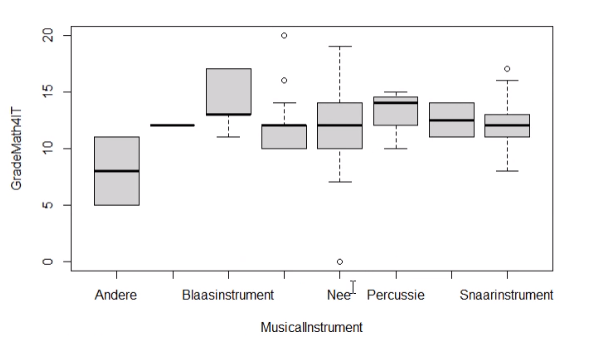
\includegraphics[scale=0.5]{../rapport/img/1.PNG}

4.2 De relatie tussen de muziekopleidingsmethode en de punten van POD1.\newline
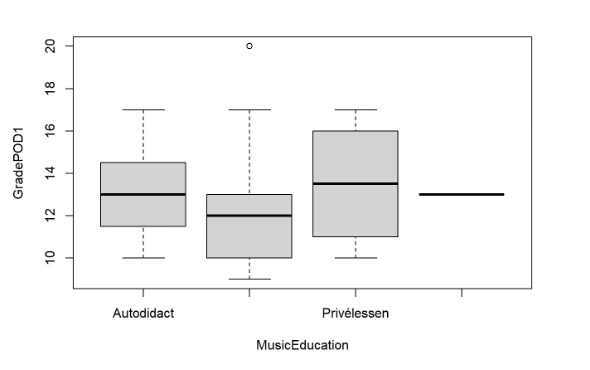
\includegraphics[scale=0.5]{../rapport/img/2.PNG}

4.3 Het verband tussen het kunnen lezen van partituren en de scores van wiskundig gerelateerde vakken doorheen het middelbaar. \newline
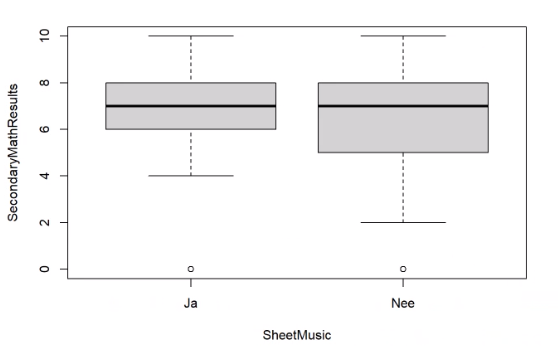
\includegraphics[scale=0.5]{../rapport/img/3.PNG}

4.4 De samenhang van het aantal jaar dat een individu al muzikaal actief is en de voorbereiding die genomen wordt bij een wiskundig gerelateerde test.\newline
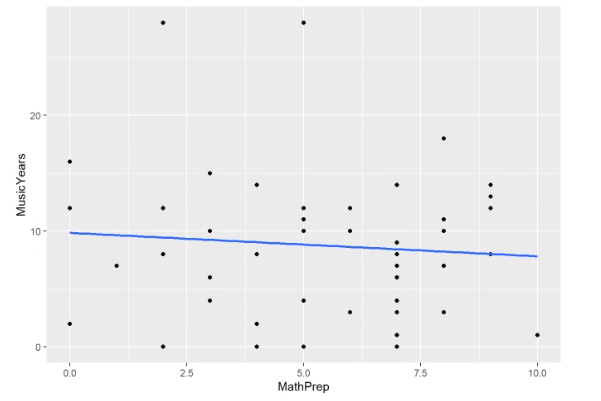
\includegraphics[scale=0.5]{../rapport/img/4.PNG}

4.5 Data met betrekking tot de berekeningen.\newline
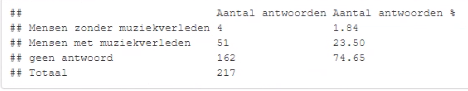
\includegraphics[scale=0.5]{../rapport/img/5.PNG}

\section{Analyse resultaten}

Grafiek 4.1 toont het type instrument dat men bespeelt indien men dit doet en het verband met de behaalde score op Math4IT. Dit toont aan dat er een klein voordeel te bemerken valt bij personen die een instrument bespelen. De mediaan ligt meermaals hoger bij personen die een instrument bespelen. 

De grafiek van 4.2 toont een overzicht van de scores op POD1. Hier valt op dat personen die autodidact en via privélessen een muziekinstrument leren bespelen hoger scoren dan personen die muziekschool of deeltijds kunstonderwijs als opleiding hebben. Alhoewel zich hier ook de uitschieter onder bevind met een perfecte score. Er was echter wel te weinig data om hier in lijn van het onderzoek een conclusie te bekomen. Het overgrote deel van de deelenemers heeft hier geen antwoord gegeven in verband met hun opleiding op muzikaal vlak indien er geen was.

Afbeelding 4.3 wijst in het voordeel van mensen die kunnen partituren lezen bij hun scores op wiskundige vlakken in het middelbaar. De mediaan ligt bij beiden op gelijke hoogte evenals hun bovengrens maar de ondergrens ligt lager bij personen die geen partituren kunnen lezen.

De voorlaatste afbeelding 4.4 toont geen duidelijk verband aan tussen hoeveel jaar een individu al muzikaal actief is en de hoeveelheid voorbereiding die het individu treft voor een wiskundige test. De gegevens zijn meer verspreid. Dit kan echter zoals zichtbaar in afbeelding 4.5 ook liggen aan het feit dat er drie op de vier leerlingen hier niet op geantwoord heeft en de data geen accurate representatie kan zijn van onze steekproef.

\section{Conclusie}

Door de dataset met beperkte bruikbare info kunnen de berekeningen niet als een accurate respresentatie van de steekproef gelden. Hierdoor kan maar een deel van de onderzoeksvraag beantwoord worden. Personen die een instrument bespelen gaan een klein aantal punten hoger scoren dan personen die dit niet doen. Onder de scores van het middelbaar was het wel zichtbaar dat personen die muzikaal actief waren betere scores haalden. Het andere deel van de data kan niet respresentatief gebruikt worden. Er is wel degelijk een verband tussen personen die muzikaal actief zijn en betere scores op wiskundig gebied. De mediaan van zowel de groep die een instrument bespeelt als de groep die dit niet doet ligt ongeveer op gelijke hoogte maar de spreiding van de scores ligt wel dichter bijeen bij de groep die muzikaal actief is. Muzikaal actief zijn kan dus positieve effecten hebben op het wiskundige grondgebied meer bepaald de wiskundige geletterheid. Er moet echter meer data verzameld worden om deze vraag accurater te kunnen beantwoorden. 

%------------------------------------------------------------------------------
% Referentielijst
%------------------------------------------------------------------------------
% TODO: de gerefereerde werken moeten in BibTeX-bestand ``bibliografie.bib''
% voorkomen. Gebruik JabRef om je bibliografie bij te houden en vergeet niet
% om compatibiliteit met Biber/BibLaTeX aan te zetten (File > Switch to
% BibLaTeX mode)

\phantomsection
\printbibliography[heading=bibintoc]

\end{document}
